Nelle seguenti analisi si è voluto studiare come al variare del parametro $\alpha$ variasse la scelta delle celle obiettivo da parte dei robot (si ricorda la strategia di scelta della cella descritto nella Sotto-sezione \ref{sub:robots} e della Formula \ref{math:info-gain}), ovvero come il peso introdotto da $\alpha$ fa variare l'importanza che gli agenti danno alla scelta dei cammini.
Come già detto, ci si aspetta che per valori di $\alpha$ elevati si scelgano celle il cui cammino per raggiungerle abbia un costo basso, e per valori di $\alpha$ bassi i robot scelgano principalmente in base all'utilità (e priorità) della cella.\\
\todo[inline]{conferma se le simulazioni sono davvero state fatte così oppure ricordo male. DP}
In questa parte di lavoro, sono state effettuate due tipi di analisi: in primo luogo, si sono studiati i costi dei cammini scelti durante tutta la durata della simulazione aggregando i risultati di varie simulazioni con lo stesso valore di $\alpha$; in seguito, si è scesi più nel dettaglio andando a valutare come i costi variano all'evolvere del tempo (in termini di \textit{step}) per ogni valore di $\alpha$ studiato in precedenza.
Tutte le simulazioni effettuate per queste analisi sono state eseguite nel seguente modo:
\begin{itemize}
	\item la dimensione della mappa è 30$\times$30 celle con 6 robot disposti all'esplorazione;
	\item il valore di $\gamma$ pari a 0.65 (inferito dal processo di ottimizzazione);
	\item il raggio di percezione pari a 6 celle (anche questo inferito dal processo di ottimizzazione);
	\item il raggio dei ripetitori \textit{wi-fi} pari a 3 celle, in modo da tenerlo proporzionale con la riduzione in scala della mappa rispetto alle dimensioni iniziali che si erano pensate.
\end{itemize}
Infine, per ogni valore di $\alpha$ sono state effettuate 10 simulazioni su mappe scelte casualmente da un insieme di 5 mappe pregenerate in modo \textit{randomico}, le quali non presentano casi patologici.

I risultati delle analisi aggregate sono mostrate in Figura \ref{fig:alphaVar}, in particolare nella Figura \ref{sfig:alphaVarAll} viene mostrata la media dei valori medi (in nero) e relative medie delle deviazioni standard (in rosso) dei costi dei cammini scelti al variare di $\alpha$, la linea tratteggiata rappresenta il valore massimo di deviazione standard dei costi che si ha avuto durante una simulazione.
Poiché i valori di $\alpha$ sono stati studiati con ordini di grandezza differenti (da $10^{-4}$ a $10$), è stato necessario produrre un altro grafico che si concentrasse solo sui valori di $\alpha$ piccoli, tale grafico viene mostrato in Figura \ref{sfig:alphaVar0.005}, la rappresentazione grafica segue la semantica utilizzata per il grafico precedente.
Dai grafici si nota che per valori relativamente alti di $\alpha$ il costo medio rimane pressoché costante, questo perché nel momento in cui $\alpha$ è abbastanza significativo da far pesare, anche solo in piccola parte, il costo del cammino nel calcolo dell'\textit{info-gain} le celle in prossimità dell'agente saranno quelle che tipicamente possiedono un valore di \textit{info-gain} maggiore e quindi verrano preferite dall'agente, portando a costi ridotti.
Al contempo, si può apprezzare come all'aumentare del parametro, nonsotante la media rimanga invariata, la deviazione standard e relativo massimo diminuscano evidenziando che i robot tenderanno sempre a preferire le celle più economiche da raggiungere a discapito di una loro utilità e priorità bassa.
Si può dedurre, che valori di $\alpha$ troppo elevati rendano inutili le politiche di prioritizzazione delle celle e le stretegie di gestione delle utilità, poiché gli agenti preferiranno sempre e solo la cella più economica da raggiungere.
Infine, in Figura \ref{sfig:alphaVar0.005} si può notare come per un valore di $\alpha$ pari a zero il costo venga completamente ignorato (come ci si aspetta) e quindi le celle scelte dipendono solo dalla loro utilità e priorità causando quindi gli agenti a continuare a muoversi per il territorio cercando semplicemente la cella più conveniente. 
\begin{figure}
	\subfloat[Media dei costi dei cammini scelti da parte degli agenti durante un insieme di simulazioni con un determinato valore di $\alpha$, relative deviazioni standard e massima deviazione standard presente in una simulazione. In questa figura sono rappresentati i dati relativi a tutti i valori del parametro analizzati.\label{sfig:alphaVarAll}]{
		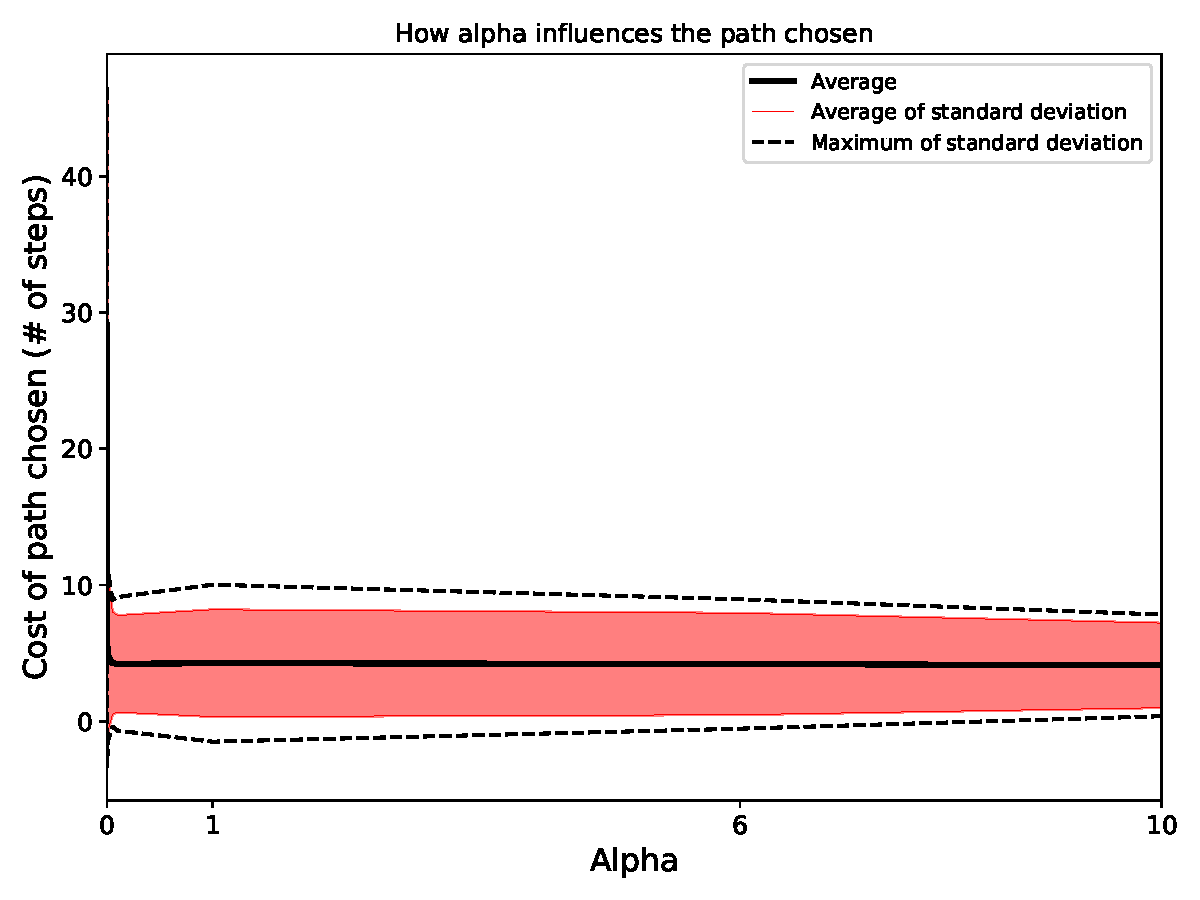
\includegraphics[width=.47\linewidth]{images/alpha_results/variation_all}
	}
	\hfill
	\subfloat[Media dei costi dei cammini scelti da parte degli agenti durante un insieme di simulazioni con un determinato valore di $\alpha$, relative deviazioni standard e massima deviazione standard presente in una simulazione. In questa figura sono rappresentati i dati relativi ai valori del parametro pari a 0, $10^{-4}$, $5\times10^{-4}$, $10^{-3}$, $5\times10^{-3}$.\label{sfig:alphaVar0.005}]{
		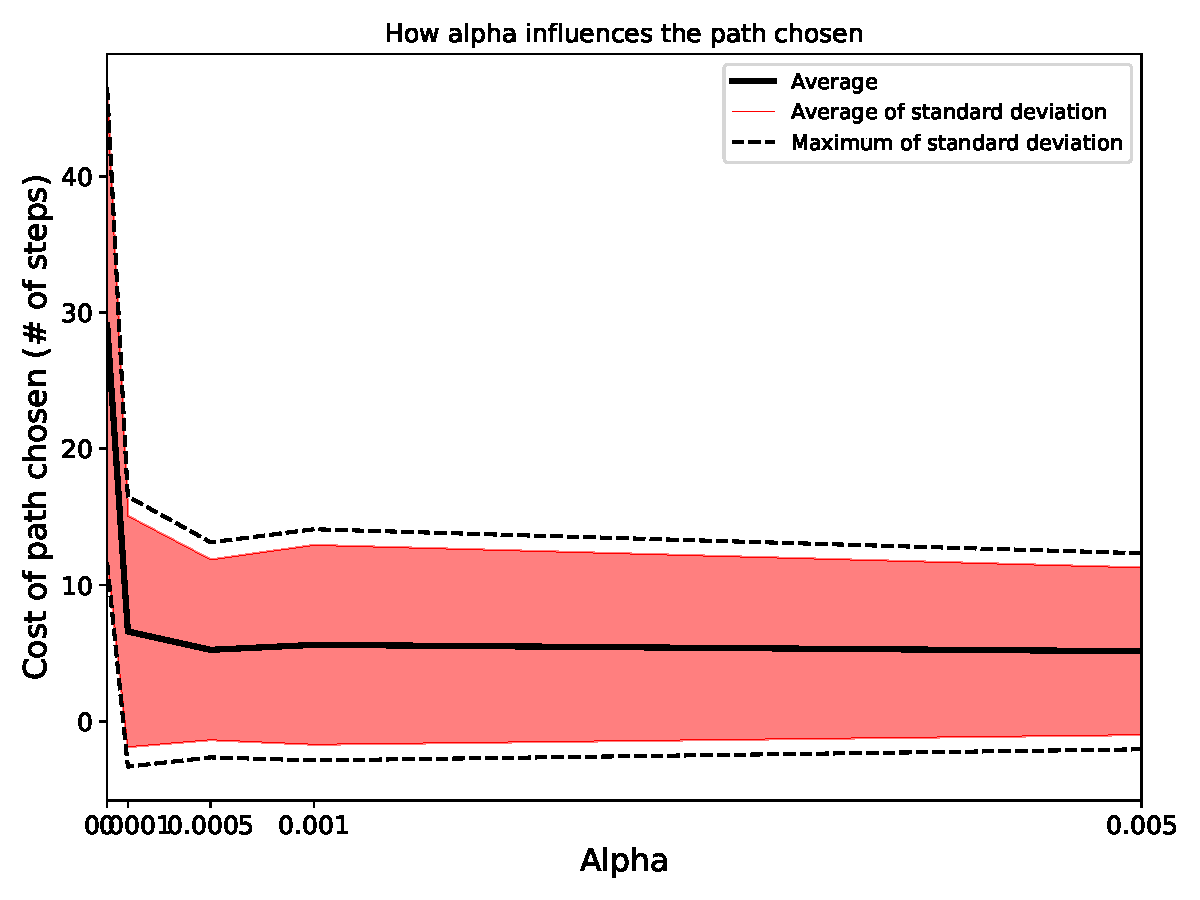
\includegraphics[width=.47\linewidth]{images/alpha_results/variation_0_005}
	}
	\caption{Per entrambi i grafici, in nero è rappresentata la media delle medie dei costi durante le singole simulazioni effettuate con un determinato valore di $\alpha$, in rosso si rappresenta la media delle deviazioni standard calcolate per ogni simulazione ed infine la riga tratteggiata indica il massimo delle deviazioni standard delle simulazioni per il relativo valore di $\alpha$.}
	\label{fig:alphaVar}
\end{figure}

Poiché le analisi precedentemente introdotte aggregano fin troppi dati, si è deciso di analizzare più nello specifico come $\alpha$ influisse nella scelta dei cammini durante la simulazione, in particolare per ogni valore di $\alpha$ preso in considerazione nella parte antecedente si è valutato per ogni \textit{step} della simulazione i costi dei cammini scelti dagli agenti.
Si sono considerati solo gli \textit{step} in cui almeno un robot ha effettuato una scelta della cella \textit{target} e se più robot hanno effettuato una scelta nello stesso \textit{step}, si è considerata la media di essi; tale studio è stato effettuato aggregando le varie simulazioni per lo stesso valore del parametro. 
Con aggregando si intende andando a valutare contemporaneamente per ogni \textit{step} cosa è successo durante le simulazioni.
I grafici per alcuni valori di $\alpha$ che sono stati ritenuti significativi sono stati riportati in Figura \ref{fig:alphaOverTime}, invece, per i grafici che si riferiscono agli altri valori si rimanda all'Appendice \ref{apx:alpha}; infine, si fa presente che per rendere i grafici leggibili sono stati accorpati i valori dei costi per intervalli di 100 \textit{step} l'uno, di conseguenza si rappresenta la media (evidenziata dalla curva colorata) e in nero gli \textit{errorbar} dati dalle relative deviazioni standard.
Dai grafici si nota come per un valore di $\alpha$ pari a zero (Figura \ref{sfig:alphaCost0}) i costo medio rimane sempre elevato e vi è un'alta varianza attorno a tale valore; come detto in precedenza, con tale valore gli agenti scelgono la cella in base alla sua utilità e priorità ignorando completamente i costi, di conseguenza tenderanno a muoversi per lunghe distanze attraverso il territorio portandole a dover ripercorre tratti di strada più volte.
Tale affermazione viene ampiamente sostenuta dall'evoluzione che ha il grafico preso in considerazione, dove il costo varia ampiamente e, come vedremo in seguito, l'epslorazione completa dell'area richiede molto più tempo del necessario.
Per quanto riguarda, invece, un valore di $\alpha$ pari a $10^{-2}$, si faccia riferimento alla Figura \ref{sfig:alphaCost0.01}, si può notare come i tempi di esplorazione diminuiscono significativamente e anche i costi sno in media molto più bassi, tale risultato accredita ulteriormente l'affermazione precedente.
In aggiunta si sottolinea che per valori relativamente poco più alti, tali costi diminuiscono in maniera ancora più significativa (si veda in Appendice la Figura \ref{sfig:alpha0.05}).
Per quanto concerne valori di $\alpha$ pari a 6 e 10 (rispettivamente in Figura \ref{sfig:alphaCost6} e \ref{sfig:alphaCost10}) si nota come il costo medio diminuisce ulteriormente solo per aumentare (come già succedeva per valori pari a $10^{-2}$ e superiori) durante le ultime fasi dell'esplorazione dove si suppone che siano rimaste solo le celle con utilità molto bassa o accerchiate da celle di difficile attraversamento che hanno scoraggiato la loro scelta da parte degli agenti finché avevano a disposizione una scelta più ampia.
Al contempo, si può notare come la deviazione standard per un valore del parametro pari a 6 sia minore rispetto ad un valore pari a 10, si può supporre che questo sia il motivo principale per cui il processo di otimizzazione abbia optato per un valore di $\alpha$ intermedio tra i due.\\
Per concludere, sono stati messi a confronto i costi medi dei percorsi scelti durante ogni simulazione, confrontando complessivamente i dati analizzati separatamente in precedenza.
I risultati sono proposti in Figura \ref{fig:alphaComparison}, dove si nota come per un valore del parametro pari a 0 i costi sono estremamente più alti e questo implica tempi di completamente dell'esplorazione maggiori, in aggiunta per valori di $\alpha$ molto bassi la media dei costi iniziali è significativamente più alta rispetto agli altri valori.
Infine, si nota come per valori di $\alpha$ pari ad uno e sei i tempi di eplsorazione finiscano leggermente in anticipo rispetto a quelli richiesti dagli altri valori.

\begin{figure}
	\begin{tabular}{cc}
		\subfloat[Effetto di un valore del parametro $\alpha$ pari a 0 nella scelta della cella obiettivo in base al costo del cammino.\label{sfig:alphaCost0}]{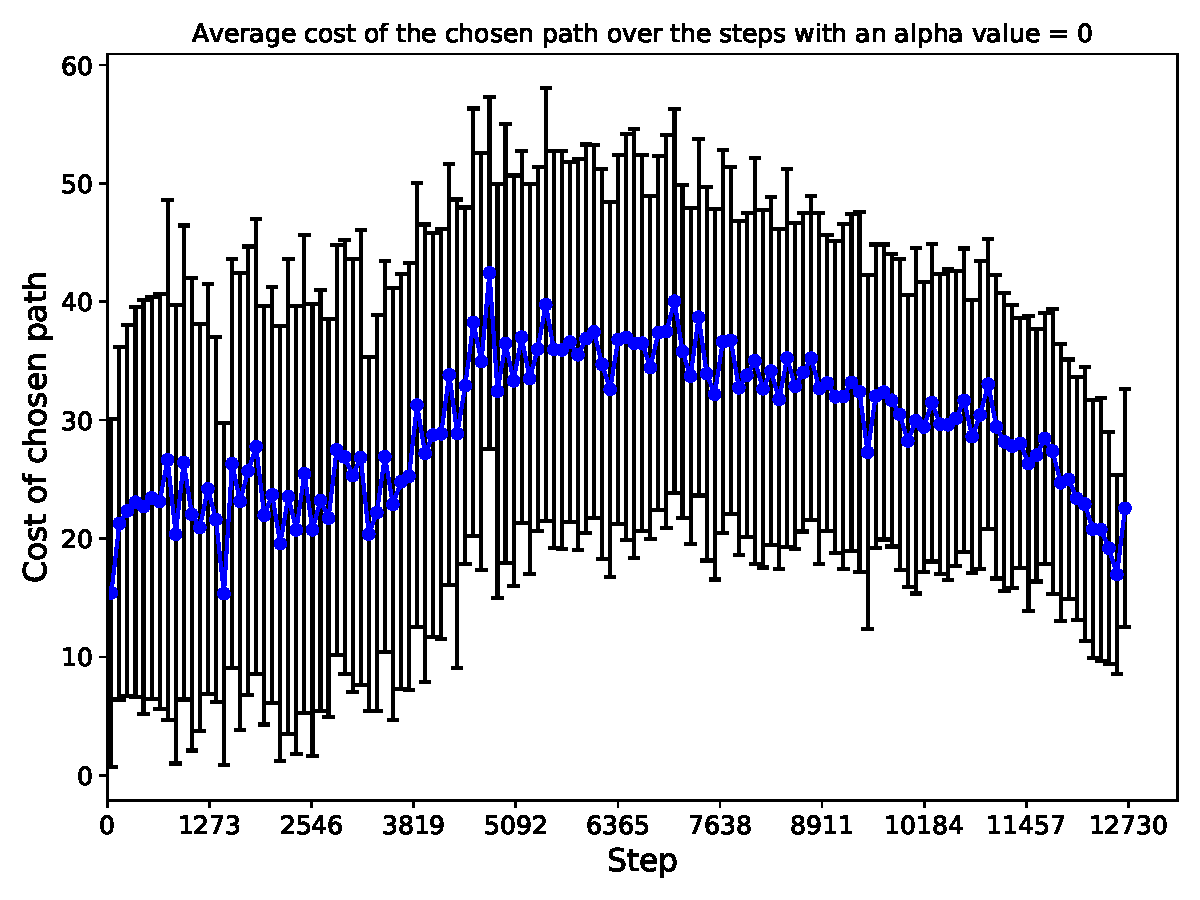
\includegraphics[width = .5\textwidth]{images/alpha_results/cost_alpha_0}} &
		\subfloat[Effetto di un valore del parametro $\alpha$ pari a 0.01 nella scelta della cella obiettivo in base al costo del cammino.\label{sfig:alphaCost0.01}]{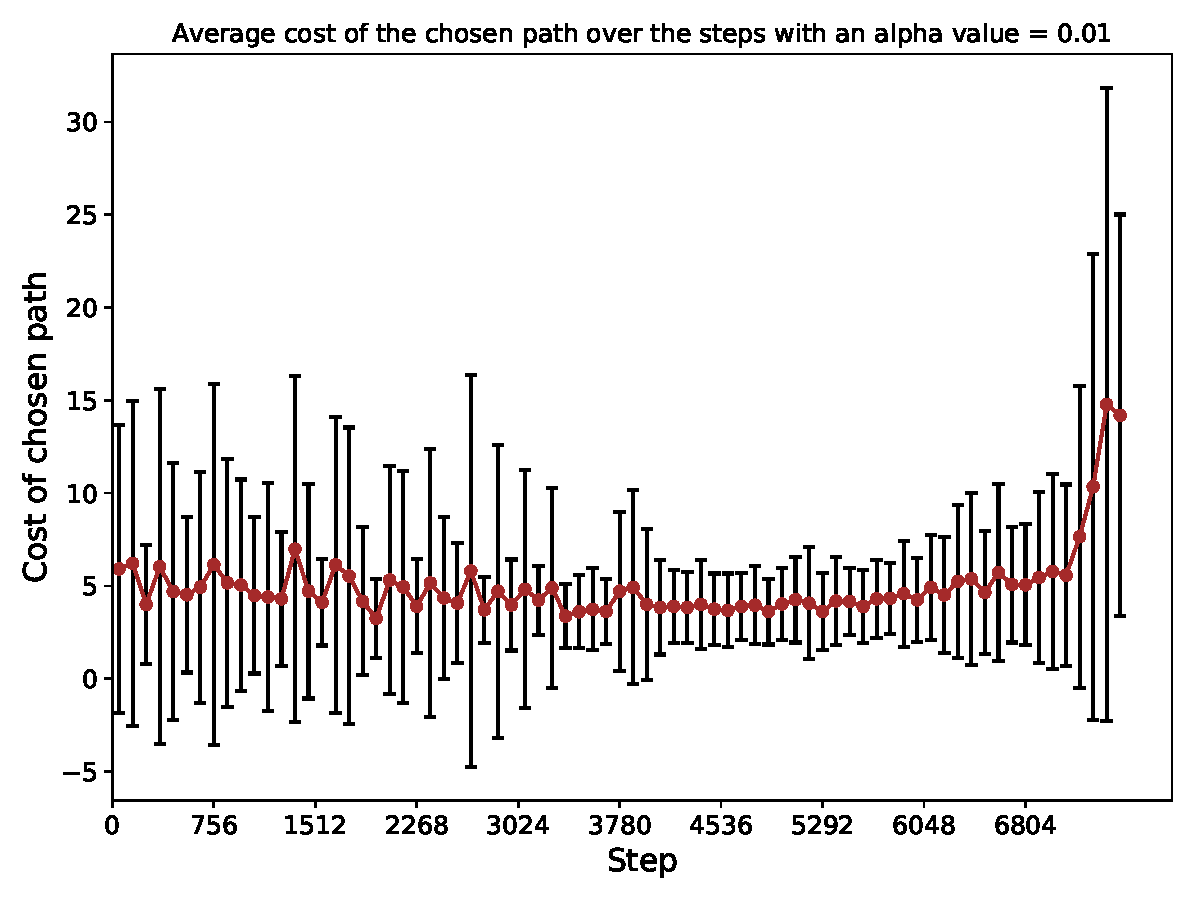
\includegraphics[width = .5\textwidth]{images/alpha_results/cost_alpha_0_01}}\\
		\subfloat[Effetto di un valore del parametro $\alpha$ pari a 6 nella scelta della cella obiettivo in base al costo del cammino.\label{sfig:alphaCost6}]{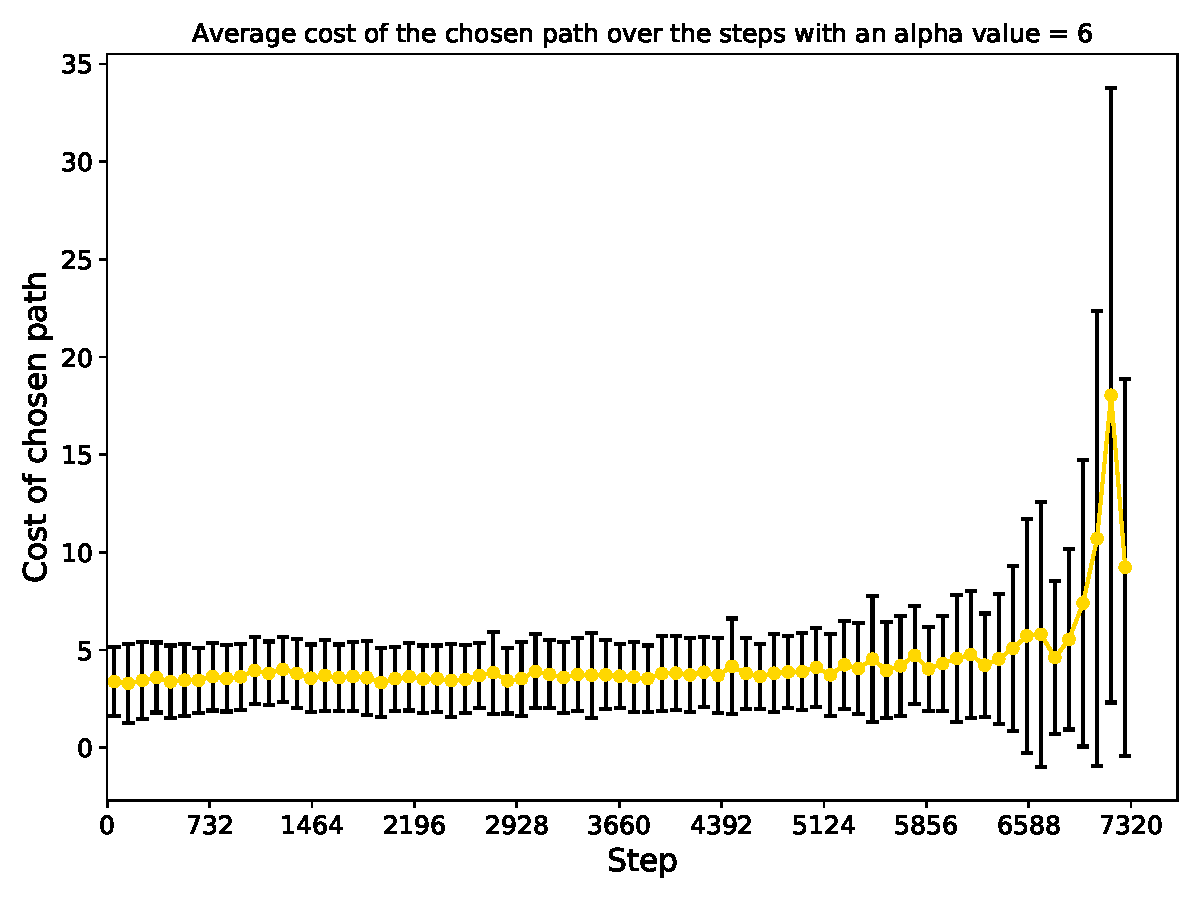
\includegraphics[width = .5\textwidth]{images/alpha_results/cost_alpha_6}} &
		\subfloat[Effetto di un valore del parametro $\alpha$ pari a 10 nella scelta della cella obiettivo in base al costo del cammino.\label{sfig:alphaCost10}]{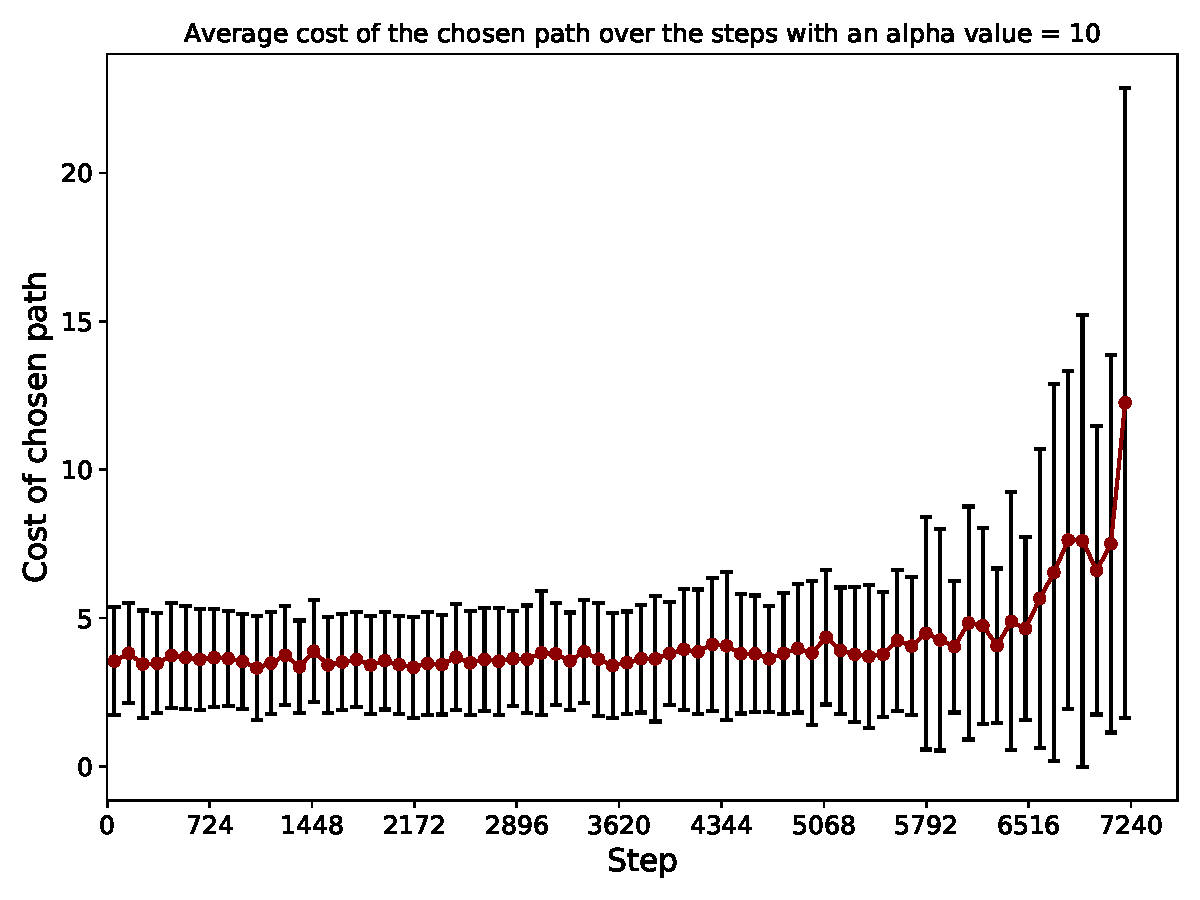
\includegraphics[width = .5\textwidth]{images/alpha_results/cost_alpha_10}}
	\end{tabular}
	\caption{In colore si denota la media dei costi dei cammini per raggiungere la cella scelta, i valori sono stati calcolati aggregando le scelte effettuate durante intervalli di 100 \textit{step}; in nero gli \textit{errorbar} relativi alla media determinati dalla deviazione standard.}
	\label{fig:alphaOverTime}
\end{figure}

\begin{figure}
	\centering
	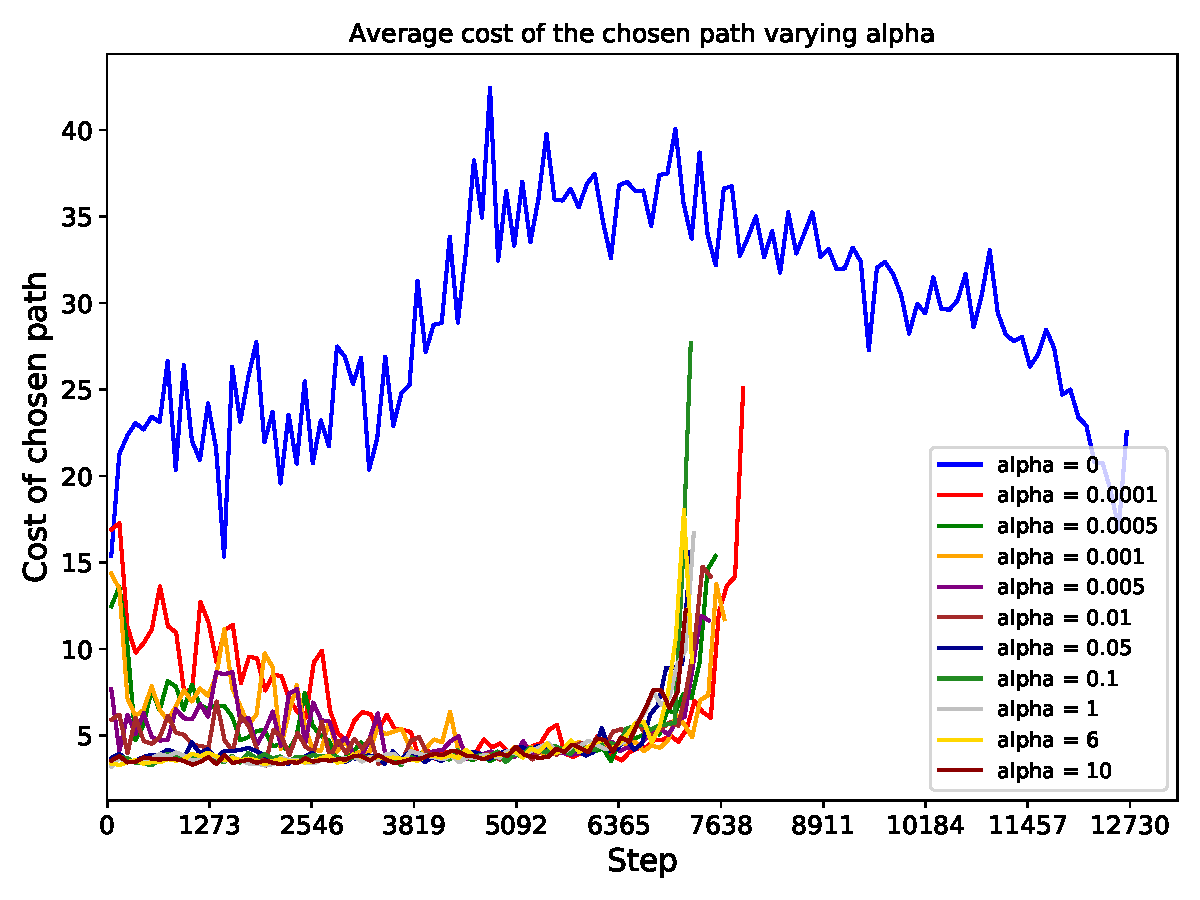
\includegraphics[width=0.9\linewidth]{images/alpha_results/comparison}
	\caption{Confronto tra la media dei costi dei cammini durante la simulazione per diversi valori di $\alpha$, anche in questo caso la media è stata calcolata in intervalli di 100 \textit{step}.}
	\label{fig:alphaComparison}
\end{figure}
